
\chapter{Banco Ottico}
\section{Introduzione}
\subsection{Scopo dell'esperimento e metodo in breve}

L'esperimento si compone di tre parti. Nella prima, si verifica la validità della Legge di Snell e la reversibilità del cammino ottico: dato un raggio luminoso attraversante un semi-cilindro in plexiglass, misuriamo l'angolo di incidenza $\theta_{rifrazione}$ ed il corrispondente  angolo di rifrazione $\theta_{rifrazione}$. Sempre grazie alla legge di Snell si ricerca la miglior stima dell'indice di rifrazione del plexiglass $n$.
\\


Nella seconda parte, si ricerca $n$ studiando l'angolo di deviazione minima $\delta_{min}$ di un prisma a base triangolare e di un prisma a base trapezoidale. Inoltre, si ricerca la distanza di cui viene traslato il raggio, che arriva con un certo angolo di incidenza $\theta$, quando passa per due superfici parallele.
\\

Infine si verifica la legge dei punti coniugati tramite la misura delle distanze $p$ e $q$ e la validità dell'ingrandimento ottico $M$. 

\subsection{Strumenti}
In questa tabella vengono riassunti gli strumenti rivelatori utilizzati, con le relative precisioni, e il set-up dell'esperimento.
\begin{center}
\begin{tabular}{c|c}
Strumento & Precisione \\
\midrule
Piatt. Graduata & $\pm 1 grado $ \\
Metro & $\pm 1 mm $\\
\end{tabular}
\end{center}

Per le prime due parti dell' esperimento, il proiettore è stato impostato sulla modalità a singolo raggio luminoso e successivamente sulla modalità oggetto per la terza e ultima parte. 
Il proiettore, insieme alla piattaforma girevole graduata, alle lenti ed a uno schermo bianco, può scorrere liberamente lungo una rotaia, permettendo di modificare le distanze tra gli oggetti a piacimento.

\section{Reversibilità del cammino luminoso}

Tutte le misure seguenti sono espresse in gradi.


\begin{table}
\center
\begin{tabular}{c|c||c|c}
 \multicolumn{2}{c}{\textit{Faccia piana}} &
\multicolumn{2}{c}{\textit{Faccia curva}} \\
$\theta_{incidenza} $ & $\theta_{rifrazione} $ &$\theta_{incidenza} $ & $\theta_{rifrazione} $\\
\midrule
 10 & 7 & 7 & 10 \\
15 & 10 & &\\
20 & \textbf{13.5} & 13.5 & 20\\ 
25 & \textbf{16.5} & & \\
30 & 20 & 30 & 20\\
40 & 26 & 26 & 40\\
35 & 23 & &\\
45&  \textbf{28.5} & & \\
\end{tabular}
\caption*{Misure in gradi}
\end{table}


Raccolti i valori degli angoli di incidenza e dei corrispondenti angoli di rifrazione, possiamo calcolare la miglior stima di $n$.
La legge di Snell esprime la relazione che lega gli indici di rifrazione dei due materiali attraversati dal raggio luminoso, e i seni degli angoli di incidenza e rifrazione:

\begin{center}
$n_1 sin\theta_1 = n_2 sin\theta_2$
\end{center}

Poiché $n_a \simeq1 $ ( indice di rifrazione dell'aria ), si ricava:

$$n_2 = \frac{sin\theta_1}{sin\theta_2}$$

Nell'elaborazione dei dati, abbiamo selezionato solo le coppie di misure cui corrispondesse un errore relativo percentuale minore del 6\%, al fine di avere una stima più precisa del valore vero di $n$.

\begin{center}
\begin{tabular}{c|c|c|c|c|c}
\textbf{$\theta_1$} & 25 & 30 & 40 & 35 & 45\\
\midrule
\textbf{$\theta_2$} & 16.5 & 20 & 26 & 23 & 28.5\\
\midrule
\textbf{$n_i$} (*) & 1.489 & 1.462 & 1.468 & 1.468 & 1.482\\
\end{tabular}\\

\end{center}

(*) in questo caso abbiamo tenuto un numero superiore di cifre significative, in quanto si tratta di calcoli intermedi 
%Ripensare alle cifre significative

$$\overline{n} = \frac{\displaystyle\sum\limits_{i=1}^N n_i}{N} = 1.474 $$

$$\sigma_n = \sqrt{\frac{\sum_{i=1}^N n_i}{N-1}} = 0.01$$

$$\sigma_{\overline{n}} = \frac{\sigma_n}{\sqrt{N}} = 0.004$$

$$n_{best} = 1.474  \pm 0.004 $$

%Cifre significative incertezza diverse da cifre significative misura!

\section{Misura dell'angolo di deviazione minima}


L'angolo di deviazione minima ($\delta_{min}$) è il più piccolo angolo misurato facendo incidere un fascio di luce sulla faccia di un prisma (con inclinazione variabile) e misurando l'ampiezza dell'angolo rifratto. Nel nostro esperimento abbiamo utilizzato due prismi: uno con base un triangolo equilatero e l'altro un trapezio rettangolo.
\\

In tabella sono riportati i valori trovati per ogni misurazione dell'angolo rifratto. Per aumentare il livello di precisione, abbiamo raccolto i dati relativi agli angoli di deviazione minima per ogni faccia di prisma a base triangolare, identificando ogni misurazione con il numero dello spigolo compreso tra le facce colpite e il verso di percorrenza della luce.
\\

Per ovvie ragioni geometriche, nel caso del prisma a base trapezoidale (è presente un solo angolo acuto, di 45 gradi) è stato impossibile effettuare misure riferite a vari vertici.

\begin{center}
\begin{tabular}{|c | c | c|}
\hline
Spigolo & $\delta_{min}$ (andata) & $\delta_{min}$ (ritorno)\\
\hline
\multicolumn{3}{|c|}{\textit{Prisma a base triangolare}} \\
\hline
1 & 41 & 31\\
2 & 43 & 39\\
3 & 41 & 41\\
\hline
\multicolumn{3}{|c|}{\textit{Prisma a base trapezoidale}} \\
\hline
1 & 28 & 21\\
\hline
\end{tabular}
\end{center}

$$\overline{\delta}_{min} = \frac{\displaystyle\sum\limits_{i=1}^6 \delta_i}{6} = 1.52$$

%Angolo deviazione minima, immagine
\subsection{Analisi dei dati}

\section{Lenti sottili}
\
Nell'ultima parte dell'esperimento, si verifica la validità della legge dei punti coniugati,
$$ \frac{1}{f} = \frac{1}{q} + \frac{1}{p} $$
\textit{p: distanza sorgente-lente}
\textit{q: distanza lente-schermo}
\textit{d: diametro circonferenza proiettata}

In tabella sono riportati sulla destra le misure effettuate con lente di focale $f=100 mm$, a sinistra con lente di focale $f=200mm$. Tutti i valori sono in cm.

\begin{center}
\begin{tabular}{*{3}{c|}*{3}{|c}}
p & q &d &p &q&d\\
\midrule
13.5 & 36.5 & 5.5 & 73.4 & 26.6 & 0.7\\
36.2 & 13.8 & 0.8 & 26.4 & 73.6 & 5.5\\
\midrule
18.0 & 22.0 & 2.5 & 61.5 & 28.5 & 0.9\\
22.0 & 18.0 & 2.1 & 28.1 & 61.9 & 4.8\\
\end{tabular}
\end{center}

Per verificare la validità, rappresentare su un grafico i punti ($\frac{1}{p};\frac{1}{q})$ e verificare che i punti sono disposti lungo una retta. 
\\
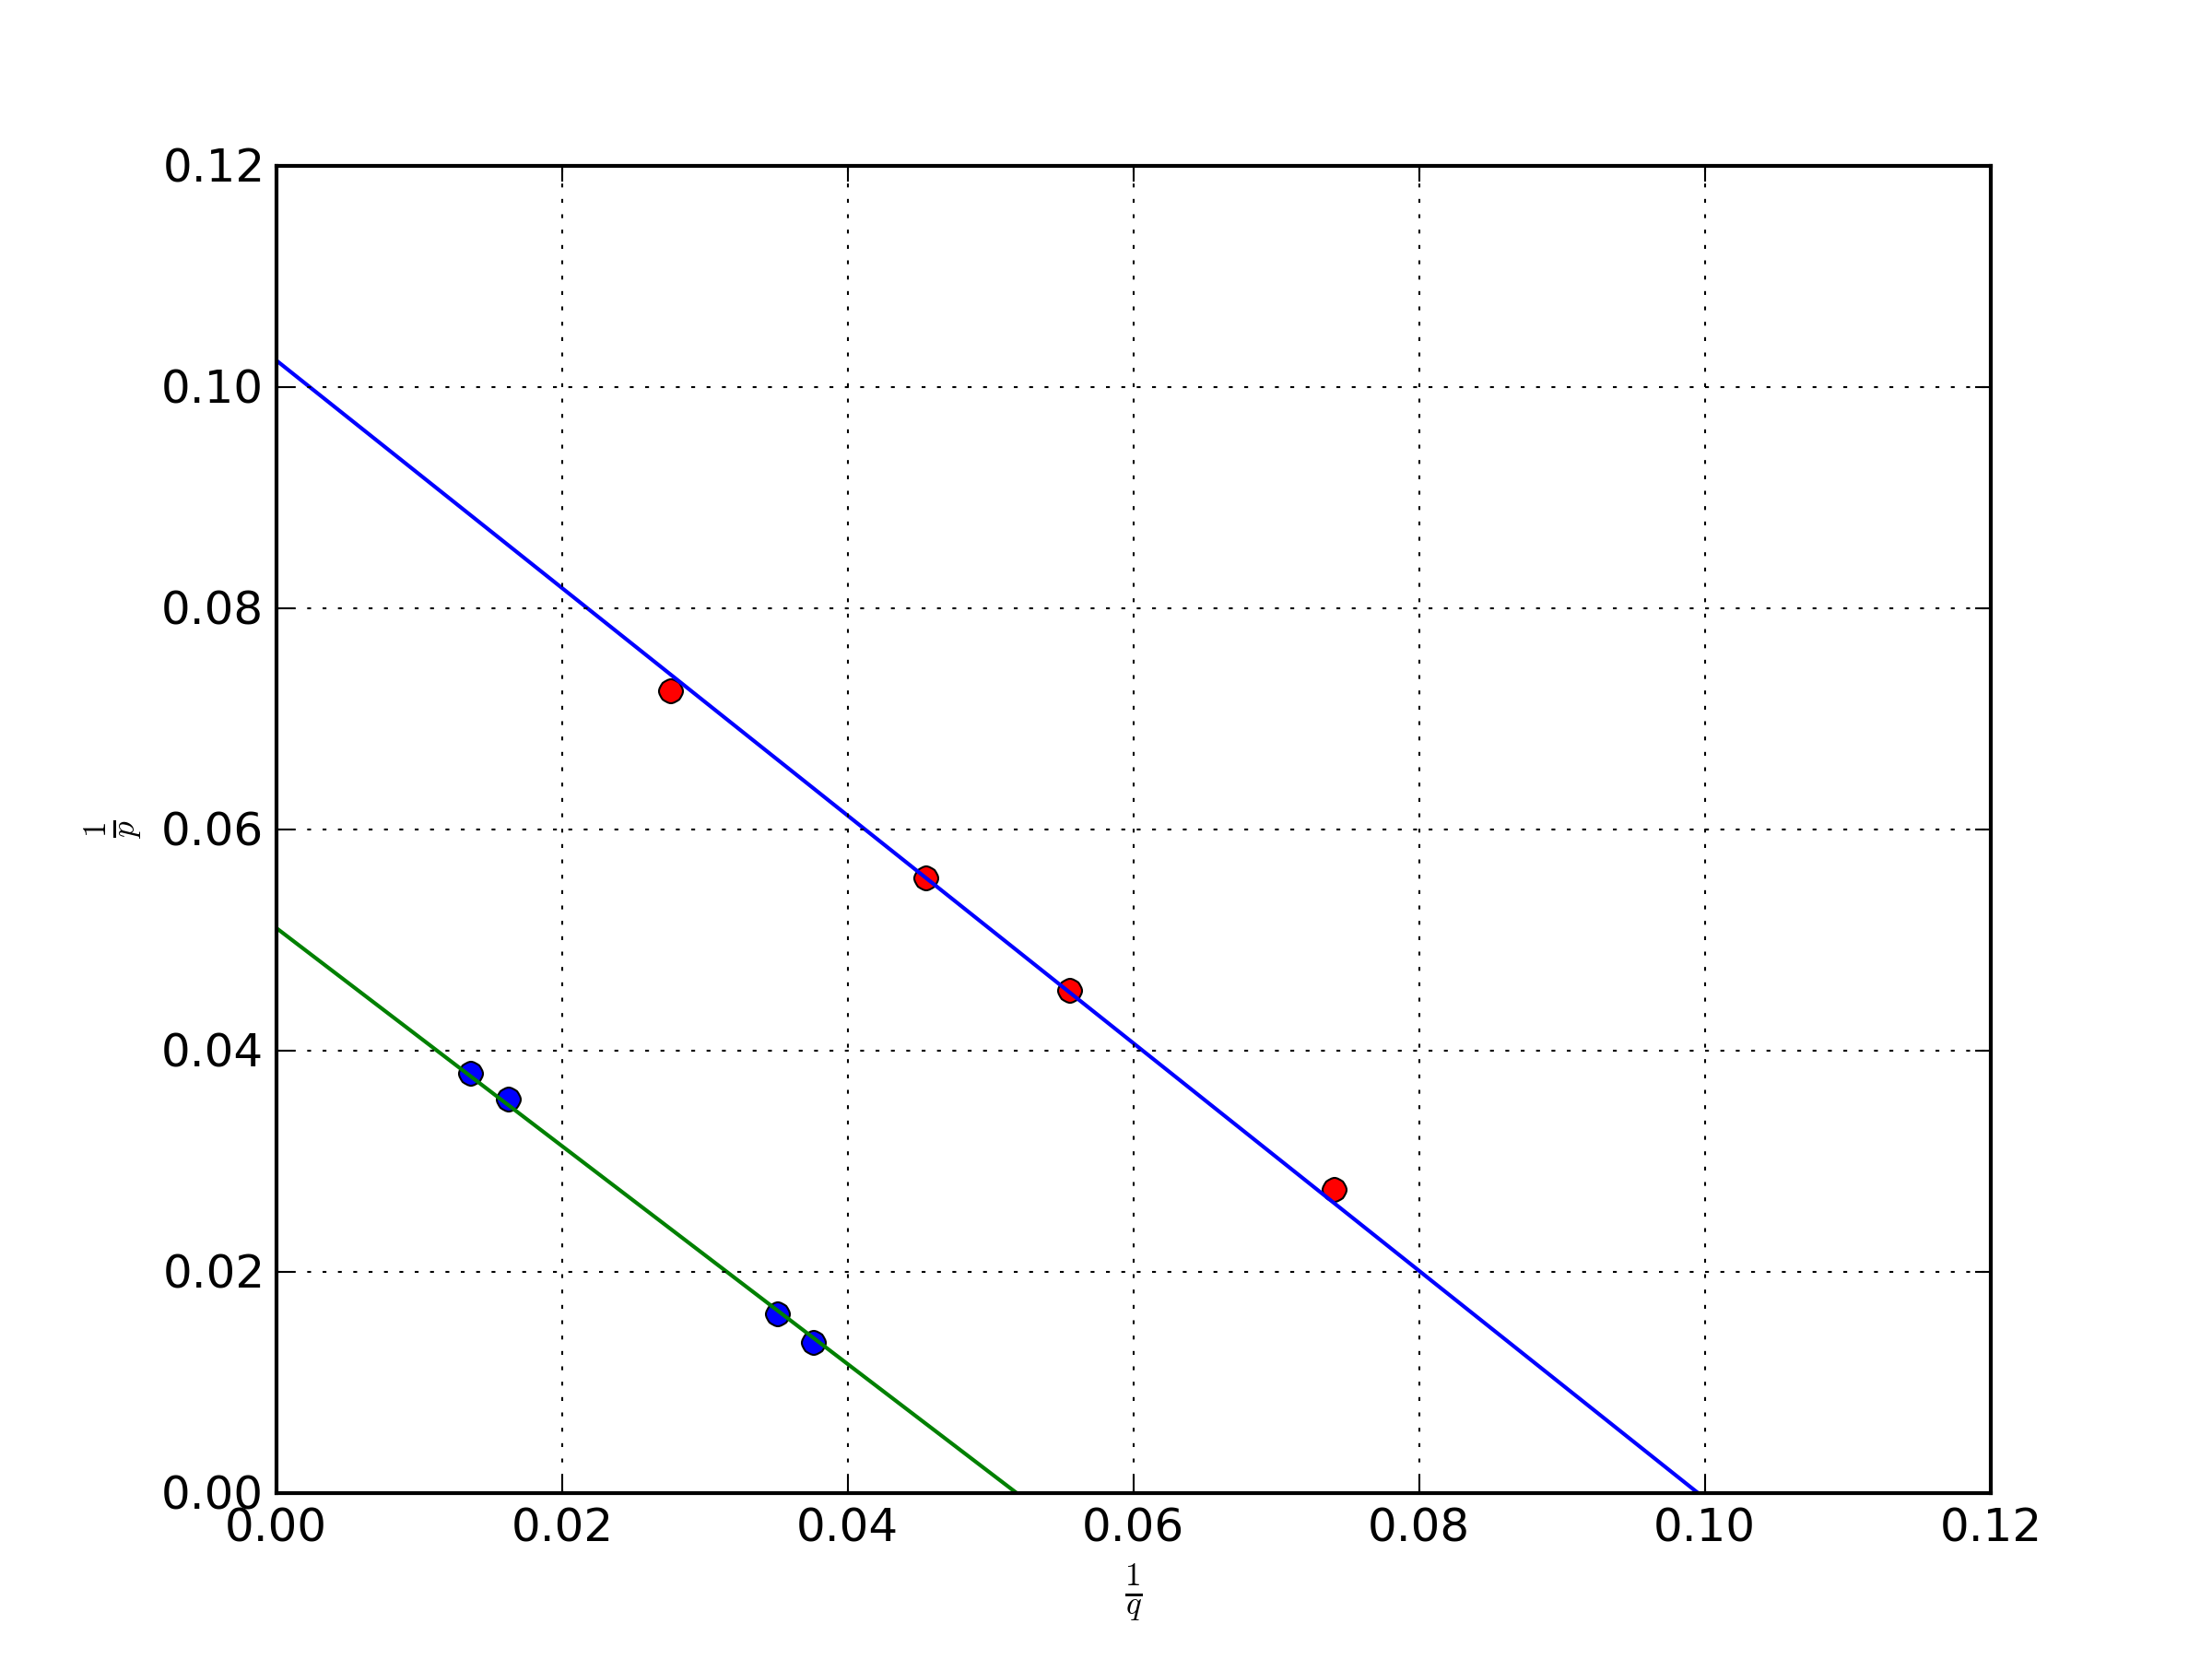
\includegraphics[scale=0.75]{../grafici/ottica}

L'intecetta trovata è $q_1 = 0.1024$ e $q_2 = 0.05108$.
Ricaviamo i valore della focale $f = \frac{1}{q}$. $f_{1} = 9.76\  cm$ e $f_{2} = 19.57\ cm$. 

L'incertezza sulla focale è data dall'espressione:
$$\delta f = \sqrt{\frac{q^4(\delta p)^2 + p^4(\delta q)^2}{(p+q)^2}}$$

ottenuta tramite il metodo delle derivate parziali.

$$\delta f_{1} = \pm 2.66\ cm $$ 
$$ \delta f_{2} = \pm 5.43\ cm $$



